\documentclass{article}

\usepackage{fancyhdr}
\usepackage{mathtools}
\usepackage{amsmath}
\usepackage{amssymb}
\usepackage{amsfonts}

\pagestyle{fancy}

\author{
  Robin Touche \\
  \and
  Fredrik Bredmar
}

\title{Machine Learning Homework 4}

\begin{document}

\maketitle

\subsection*{1.1}
\paragraph{a)}

Only graph (1).

\paragraph{b)}

Each layer may only have outgoing edges directed to the next layer.
That is no cycles are allowed, no edges going backwards between layers and
no edges between units within a single layer.

\subsection*{1.2}

By definition the current network looks like this

\begin{align}
  y = \frac{1}{2}\mathbf{w}_1^T \mathbf{x} + \frac{1}{2}\mathbf{w}_2^T \mathbf{x}
\end{align}

We want to create a network that looks like

\begin{align}
  y = \mathbf{w}_3^T \mathbf{x}
\end{align}

If we combine these equations we get the following expression to solve.

\begin{align}
  \nonumber \mathbf{w}_3^T \mathbf{x} &= \frac{1}{2}\mathbf{w}_1^T \mathbf{x} + \frac{1}{2}\mathbf{w}_2^T \mathbf{x} \Leftrightarrow\\
  \mathbf{w}_3^T &= \frac{1}{2}\mathbf{w}_1^T + \frac{1}{2}\mathbf{w}_2^T \Leftrightarrow\\
  \nonumber \mathbf{w}_3 &= \frac{1}{2}\mathbf{w}_1 + \frac{1}{2}\mathbf{w}_2
\end{align}

So clearly $f(\mathbf{w}_1,\mathbf{w}_2) = \frac{1}{2} \mathbf{w}_1 + \frac{1}{2}\mathbf{w}_2$ which definitely is linear.
So we can get the exact same predictions in a single feed-forward network.
\subsection*{1.3}

We calculate the gradient of $E = \frac{1}{2} \left(t - y \right)^2$ with regards
to $\mathbf{w}$, multiply by our learning rate and subtract this from the new
weight. So the new weights become

\begin{align}
  w_i^+ = w_i + \frac{\partial E}{\partial w_i} = w_i - (t - y)
\end{align}

\subsection*{1.4}

\paragraph{a}

\begin{align}
  \frac{\partial E}{\partial z_k} = \frac{\partial y_k}{\partial z_k} \frac{\partial E}{\partial y_k} =
  y_k \left( 1 - y_k \right) \frac{\partial E}{\partial y_k}
\end{align}

\paragraph{b}

\begin{align}
  \frac{\partial E}{\partial z_j} = \frac{\partial y_j}{\partial z_j} \frac{\partial E}{\partial y_j} =
  \sum_k \frac{\partial E}{\partial z_k}\frac{\partial z_k}{\partial y_j} y_j \left( 1 - y_j \right) =
   y_j \left( 1 - y_j \right) \sum_k \frac{\partial E}{\partial z_k}w_{jk}
\end{align}

\paragraph{c}

\begin{align}
  \frac{\partial E}{\partial w_{jk}} = \frac{\partial z_k}{\partial w_{jk}} \frac{\partial E}{z_k} =
  y_j \frac{\partial E}{\partial z_k}
\end{align}

\paragraph{d}

\begin{align}
  \frac{\partial E}{\partial w_{ij}} = \frac{\partial z_j}{\partial w_{ij}} \frac{\partial E}{z_j} =
  y_i \frac{\partial E}{\partial z_j}
\end{align}

\subsection*{2.1}

For the weight decay we have
$E = \frac{\text{weight decay}}{2}\sum \theta^2$ so the gradient is

\begin{align}
  \nonumber \frac{\partial E}{\partial w_i} = 2 \cdot \frac{1}{2} \text{weight decay} \cdot \theta = \text{weight decay} \cdot \theta
\end{align}

For the cross entroypy we have
$$ \mathbf{z} = \mathbf{Wx}$$
$$\frac{dz}{dw} = x, \frac{dz}{dx} = w$$
$$ y^{(i)} = \sigma(\mathbf{z^{(i)}})$$
$$E = -\frac{1}{m} \sum_{i=1}^m \sum_c^k log(y^{(i)}_c)
t_c^{(i)} $$

So the gradient for the output layer to hidden layer is
$$ \frac{\partial E}{\partial z_c} =\frac{1}{m}(y_c - t_c) $$
The gradient for the hidden layer to the input layer is then
$$\frac{\partial E}{\partial w_{c,j}} = \frac{\partial E}{\partial z_c}\frac{dz_c}{dw_{c,j}}
= \frac{1}{m}(y_c - t_c)x_j$$
\subsection*{2.2}

The code we added to the gradient function is as follows

\begin{verbatim}
  output_error = class_prob - data.targets;
  weight_diff = output_error * hid_output' / size(data.inputs,2);

  hidden_error = (model.hid_to_class' * output_error);
  hidden_error = (hid_output .* (1 - hid_output)) .* hidden_error;
  hid_weight_diff = hidden_error * data.inputs' / size(data.inputs,2);

  res.input_to_hid = model.input_to_hid .* wd_coefficient + hid_weight_diff;
  res.hid_to_class = model.hid_to_class .* wd_coefficient + weight_diff;
\end{verbatim}

net(0.1, 7, 10, 0, 0, false, 4) have training cost 2.768381.

\subsection*{2.3}

\paragraph{a}
The lowest training cost come from using a learning rate of $0.2$ with a momentum of $0.9$.
The training cost is then $1.083429$. Figure 1 show how the cost decrease over the number of iterations.


\begin{figure}[h!]
  \centering
    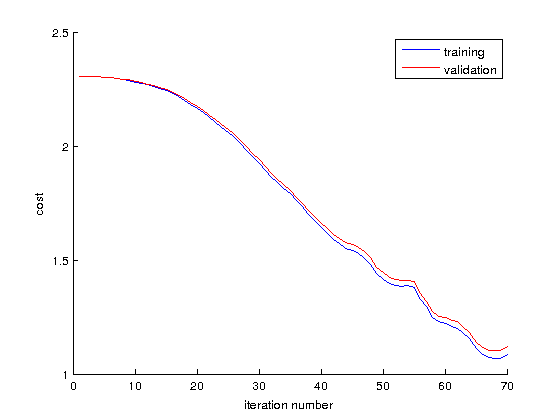
\includegraphics[width=0.5\textwidth]{pics/prob23a.png}
    \caption{Cost graph for the best case of the 14 experiments.}
\end{figure}

\paragraph{b}

The best run is with a momentum ($0.9$).

\paragraph{c}

With a learning rate of $0.2$.

\subsection*{2.4}

\paragraph{a}

The validation cost of running net(0, 200, 1000, 0.35, 0.9, false, 100) is
$0.430185$. Figure 2 show how the cost have a minimum prior to the end of the iterations.

\begin{figure}[h!]
  \centering
    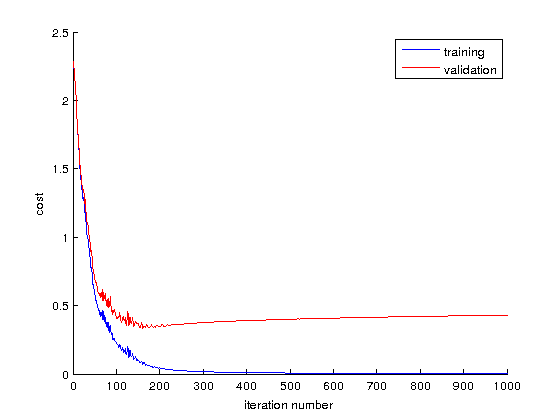
\includegraphics[width=0.5\textwidth]{pics/prob24a.png}
    \caption{Cost graph for net(0, 200, 1000, 0.35, 0.9, false, 100).}
\end{figure}


\paragraph{b}

With the use of early stopping we get a validation cost of $0.334505$.
The validation cost was the lowest at iteration number 161.
 From Figure 2 we can see that it should be around iteration $150$ and $200$ which indeed is correct.

\paragraph{c}

\begin{tabular}{c | c}
  Weight decay & validation cost\\
  \hline
  0 & 0.430185\\
  \hline
  10 & 22.612744\\
  \hline
  1 & 2.302585\\
  \hline
  0.0001 & 0.348294\\
  \hline
  0.001 & 0.287910\\
  \hline
  5 & 2.302858\\
\end{tabular}

A low weight decay of $0.001$ seem to work well.

\paragraph{d}

\begin{tabular}{c | c}
  Number of hidden units & validation cost\\
  \hline
  10 & 0.421705\\
  \hline
  30 & 0.317077\\
  \hline
  100 & 0.368593\\
  \hline
  130 & 0.397597\\
  \hline
  200 & 0.430185\\
\end{tabular}

Without early stopping a hidden layer of $30$ units give the lowest
validation cost.

\paragraph{e}

\begin{tabular}{c | c}
  Number of hidden units & validation cost\\
  \hline
  18 & 0.306083\\
  \hline
  37 & 0.265165\\
  \hline
  83 & 0.311244\\
  \hline
  113 & 0.313749\\
  \hline
  236 & 0.343841\\
\end{tabular}

With early stopping $37$ hidden units work best.
 Figure 3 show a run with early stopping and $37$ hidden units.

\begin{figure}[h!]
  \centering
    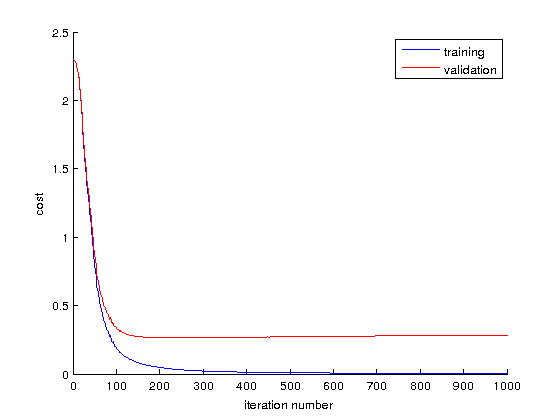
\includegraphics[width=0.5\textwidth]{pics/prob24e.png}
    \caption{Cost graph with 37 hidden units and early stopping.}
\end{figure}

\paragraph{f}

Running net(0, 37, 1000, 0.35, 0.9, true, 100) give test data error of
$0.084333$.

\end{document}
